%
% Шаблон для НИР
%

\documentclass[a4paper,12pt]{article}
\usepackage[backend=biber,sorting=none,style=gost-numeric]{biblatex} % библиография
\usepackage{mathtext} %русские буквы в формулах
\usepackage[T2A]{fontenc}
\usepackage[utf8]{inputenc}
\usepackage[english,russian]{babel}
\usepackage{amsmath}
\usepackage{fancyvrb}
\usepackage{formular}
\usepackage{setspace} % управление междустрочными интервалами
%поля документа
\usepackage[left=3cm,right=1cm,top=2cm,bottom=2cm]{geometry}

\usepackage{misccorr} % точки в конце номеров разделов, использовать перед пакетом ccaption!
\usepackage{ccaption} % изменения подписей к рисункам и табл.

\usepackage[nooneline]{caption} 
\captionsetup[table]{justification=raggedright} % заголовок таблицы выравнивается влево
\captionsetup[figure]{justification=centering,labelsep=endash} % заголовок рисунка - по центру

% отступ перед первым абзацем
\usepackage{indentfirst}
%вставка изображений
\usepackage{graphicx}
% счетчики
\usepackage{totcount}
% управление содержанием
\usepackage{tocloft}
% управление таблицами и рисунками
\usepackage{float}

%для добавления количества источников в реферат - не работает для bibtex!
\newtotcounter{citnum} %From the package documentation
\def\oldbibitem{} \let\oldbibitem=\bibitem
\def\bibitem{\stepcounter{citnum}\oldbibitem}

% окружение для листингов - с нумерацией строк слева
\DefineVerbatimEnvironment{MyCode}{Verbatim}{frame=lines,numbers=left,numberblanklines=false,framesep=5mm}

% автоматическая нумерация листингов
\newfloat{Program}{phb}{lop}
\floatname{Program}{Листинг}
\floatstyle{ruled}

\setcounter{secnumdepth}{3} % глубина нумерации до подразделов

%если нужны точки в оглавлении для разделов - раскомментируйте следующую команду
%\renewcommand{\cftsecleader}{\cftdotfill{\cftdotsep}}

\addto\captionsrussian{%
\renewcommand{\figurename}{Рисунок}%
\renewcommand{\tablename}{Таблица}%
}

% дефис в подписи к рисункам
\captiondelim{ -- } 

% Настройки для окружений с подчеркиваниями для подписей и пр.
\setFRMfontencoding{T2A}
\setFRMdfontencoding{T2A}
% thanks to A.Starikov
\setFRMfontfamily{cmr}
\setFRMdfontfamily{ptm}
\setFRMdfontsize{10pt}

% задает длину поля для подписи на титульной странице
\newFRMfield{xtitlesign}{32mm}

% поле для факультета или кафедры
\newFRMfield{fcath}{65mm}

%имя файла с библиографией в формате BibTex
\addbibresource{rbiblio.bib}

\begin{document}

% счетчики страниц, рисунков, таблиц
\regtotcounter{page}
\regtotcounter{figure}
\regtotcounter{table}

\renewcommand{\refname}{\centerline{СПИСОК ИСПОЛЬЗОВАННОЙ ЛИТЕРАТУРЫ}} 
\renewcommand{\contentsname}{\centerline{СОДЕРЖАНИЕ}} 
%\renewcommand{\refname}{Список источников}  % По умолчанию "Список литературы" (article)
%\renewcommand{\bibname}{Литература}  % По умолчанию "Литература" (book и report)

% титульная страница
\thispagestyle{empty}
\begin{center} \small
\textbf{МИНИСТЕРСТВО ОБРАЗОВАНИЯ И НАУКИ РОССИЙСКОЙ ФЕДЕРАЦИИ}\\
ФЕДЕРАЛЬНОЕ ГОСУДАРСТВЕННОЕ АВТОНОМНОЕ ОБРАЗОВАТЕЛЬНОЕ УЧРЕЖДЕНИЕ
ВЫСШЕГО  ОБРАЗОВАНИЯ\\
«Национальный исследовательский ядерный университет «МИФИ»\\
\textbf{Обнинский институт атомной энергетики} – \\
филиал федерального государственного автономного образовательного учреждения высшего\\
образования «Национальный исследовательский ядерный университет «МИФИ»\\
(ИАТЭ НИЯУ МИФИ)
\end{center}
%\vfill
\medskip

% Направление подготовки следует уточнять,
% магистры и бакалавры могут иметь разные наименования
\begin{center}
\begin{tabular}{rl}
Отделение & \useFRMfield{fcath}[\large Интеллектуальные кибернетические системы] \\ 
Направление подготовки & \useFRMfield{fcath}[\large Информационные системы и технологии] \\ 
\end{tabular} 
\end{center}

\vfill

\large 

\begin{center}
	Отчёт по преддипломной практике \\
	
	\medskip
	
	\textbf{\Large 
		Разработка мобильного приложения для преобразования 2D фотографий в 3D вид
	}
	
\end{center}

\vspace{1cm}

\begin{tabular*}{\textwidth}{lcr}
Студент группы ИС-Б14 & \useFRMfield{xtitlesign} & А.В.Кузнецов\\
& & \\
Руководитель & & \\
к.т.н., доцент отделения ИКС & \useFRMfield{xtitlesign} & О.А.Мирзеабасов\\
\end{tabular*}


\vfill
\large

\begin{center}
Обнинск, 2018 г
\end{center}

\onehalfspacing

\pagebreak

% реферат
\thispagestyle{empty}

\section*{\centering РЕФЕРАТ}

% возможно, кол-во источников придется вставлять вручную
\total{page} стр., \total{figure} рис., 7 ист. 

ANDROID, JAVA, МОБИЛЬНОЕ ПРИЛОЖЕНИЕ, ПОЛЬЗОВАТЕЛЬСКИЙ ИНТЕРФЕЙС, КАРТА ГЛУБИНЫ, АНАЛИЗ, 3D, АНИМАЦИЯ, GIF

Настоящая работа посвящена изучению методов получения трехмерных изображений из двумерных и разработке пользовательского интерфейса мобильного приложения для преобразования 2D фотографий в 3D вид. 

Разработанная программа дает возможность преобразовывать простую фотографию в объемную картинку, в виде GIF.


\pagebreak



\tableofcontents
% если нужно добавить "Стр." над номерами страниц - раскомментируйте следующую команду
%\addtocontents{toc}{~\hfill\textbf{Стр.}\par}

\pagebreak

\section*{\centering ВВЕДЕНИЕ}
\addcontentsline{toc}{section}{ВВЕДЕНИЕ}
Основным результатом выполнения проекта будет мобильное приложение, предназначенное для преобразования 2D изображений в 3D вид. Приложение будет распространяться с помощью его размещения в Google Play (для Android-устройств). Соответственно, в качестве основных потребителей создаваемой продукции следует рассматривать владельцев мобильных устройств, которые любят использовать свой телефон или планшет в качестве фотоаппарата. Более того, то подмножество этих пользователей, которые, помимо фотографирования, активно обрабатывают свои фото средствами мобильного устройства и активно делятся этими результатами с друзьями посредством соцсетей.

Поэтому главной целью текущей работы является изучение разработки мобильного приложения, работы алгоритма преобразования двумерных изображений в трехмерные и разработке современного, функционального и удобного пользовательского интерфейса. 

Задачи, решаемые в ходе работы:
\begin{enumerate}
	\item Установка и настройка программного продукта Android Studio ;
	\item Разработка пользовательского интерфейса мобильного приложения;
	\item Программная реализация алгоритма преобразования 2D фотографии в 3D;
	\item Тестирование стабильности и качества алгоритма преобразования 2D фотографий в 3D;
	\item Оптимизация параметров алгоритма.
\end{enumerate} % текст введения в файле intro.tex
\pagebreak

%\input{Post_zad}
\pagebreak
% первая часть

\section{Описание предметной области}
В ходе выполнения проекта, главным образом, решается задача преобразования двумерных изображений в трехмерные(GIF) на мобильных устройствах.

В последние годы заметное место в области преобразования и фильтрации изображений занимает задача преобразования двумерных изображений в трехмерные. На сегодняшний день в мире для этого разработаны различные методики, которые позволяют автоматически создавать так называемые «карты глубины» для двумерных изображений, основываясь на свойствах этого изображение и на некоторых предположениях о характере сцены. 

\subsection{Выбор архитектуры мобильного приложения}
В ходе выполнения работы были рассмотрены различные варианты для создания мобильных приложений, предназначенных для преобразования 2D изображений в 3D вид. При этом рассмотрении учитывалось, что результирующие мобильные приложения должны создаваться под операционные системы Android, а также то, что один из основных результатов работы приложения с точки зрения конечного пользователя – это возможность публикации созданного 3D-изображения в виде анимированного gif-файла в одном или нескольких аккаунтов в социальных сетях пользователя. Соответственно, можно исходить из предположения о том, что для функционирования приложения в любом случае необходим доступ к сети интернет. Максимальная унификация различных составных частей приложения между собой хотя бы на уровне исходных кодов вне зависимости от целевой платформы (Android или iOS) является дополнительным преимуществом при рассмотрении различных вариантов создания мобильных приложений.

Один из наиболее простых с технической точки зрения вариантов реализации решения, позволяющего преобразовывать 2D файлы в 3D вид, является решение, основанное на создании веб-сервиса, который предоставляет минимально необходимый пользовательский интерфейс для загрузки желаемого файла на сервер, преобразования файла на сервере и, как результат, возможность скачать получившийся файл на устройство пользователя и поделиться этим файлом в социальных сетях. При простоте архитектуры у этого решения есть один существенных недостаток – как правило, такие решения менее удобны и функциональны, чем нативные (native) мобильные приложения, разработанные специально под целевую платформу, на которой они будут функционировать.

Рассмотрим два варианта создания нативных мобильных приложений:

\begin{enumerate}
	\item Использовать наиболее популярные средства разработки и языки программирования для каждой из необходимых мобильных платформ. Создать нативное мобильное приложение, реализующее весь необходимый пользовательский интерфейс, набор сервисных функций. Портировать алгоритм преобразования графического файла из 2D в 3D для локального исполнения на мобильном устройстве. Все необходимые преобразования выполнять локально, на мобильном устройстве. Полученный результат преобразования (анимированный gif) загружать в интернет (социальные сети) по мере его готовности на мобильном устройстве.
	
	\item Использовать наиболее популярные средства разработки и языки программирования для каждой из необходимых мобильных платформ для создания нативных мобильных приложений только для реализации пользовательского интерфейса и набора сервисных функций. Алгоритм преобразования графического файла из 2D в 3D реализуется в виде серверного модуля, соответственно для преобразования выбранного файла и предварительного просмотра полученных результатов необходимо загрузить этот выбранный файл на сервер. Загрузить полученный результат с сервера и поделиться этим результатом в социальных сетях.
\end{enumerate}

Для варианта №1 для операционной системы Android необходимо:

С использованием Android Studio на языке программирования Java реализовать необходимый пользовательский интерфейс, а также весь необходимый набор сервисных функций. Необходимо адаптировать реализацию алгоритма преобразования графического файла из 2D в 3D для использования под управлением операционной системы Android (реализация на С++). Далее, с использованием механизма The Android Native Development Kit (NDK) необходимо обеспечить вызов кода, написанного на языке С++ из «классического» Android-приложения. 

Для реализации варианта №2 необходимо:

С использованием Android Studio на языке программирования Java необходимо создать нативное мобильное приложение для реализации пользовательского интерфейса и набора сервисных функций. Эта задача, в целом, является типовой и принципиальных сложностей не вызывает. Алгоритм преобразования графического файла из 2D в 3D следует реализовать в виде серверного модуля, например, для использования под управлением операционной системы Ubuntu. Это обусловлено тем, что Unix-подобные операционные системы имеют существенно более широкое распространение в Web-серверном окружении, чем Windows-сервера.

На основе проведенного исследования моно сделать следующий вывод. С точки зрения скорости, легкости и качества реализации наиболее перспективными являются вариант №2. 

Очевидным недостатком подобного решения является существенная его зависимость от скорости и надежности мобильного интернета, а также от доступности конечному пользователю оплаченного трафика. Для обхода этих ограничений предполагается исследовать возможность создания для пользователей ОС Android «самодостаточного» мобильного приложения (вариант №1), которое все необходимые действия, связанные с преобразованием файлов производит непосредственно на мобильном устройстве.


\section{Проектирование структуры приложения}

Одна из важнейших задач в ходе создания мобильного приложения, преобразовывающего 2D снимки в объемные (3D) - разработка удобного и интуитивно-понятного пользовательского интерфейса. UI/UX (user Interface, user experience) составляющая, она же пользовательский интерфейс и пользовательский опыт, является более чем просто значимым элементом современного мобильного приложения. Удобство расположения элементов управления и приятное визуальное оформление напрямую влияют на настроение пользователя при использовании продукты. Именно некачественный UI/UX-дизайн отпугивает людей от использования многих приложений в пользу их более достойных альтернатив.

На главный экран камеры (рисунок~\ref{fig:Artboard}) выведены следующие функции:

\begin{itemize}
	\item Спуск затвора;
	\item Выбор фото из галереи;
	\item Смена камеры;
	\item Управление вспышкой;
	\item Переход к настройкам и справке.
\end{itemize}

\begin{figure}[H]
	\centering
	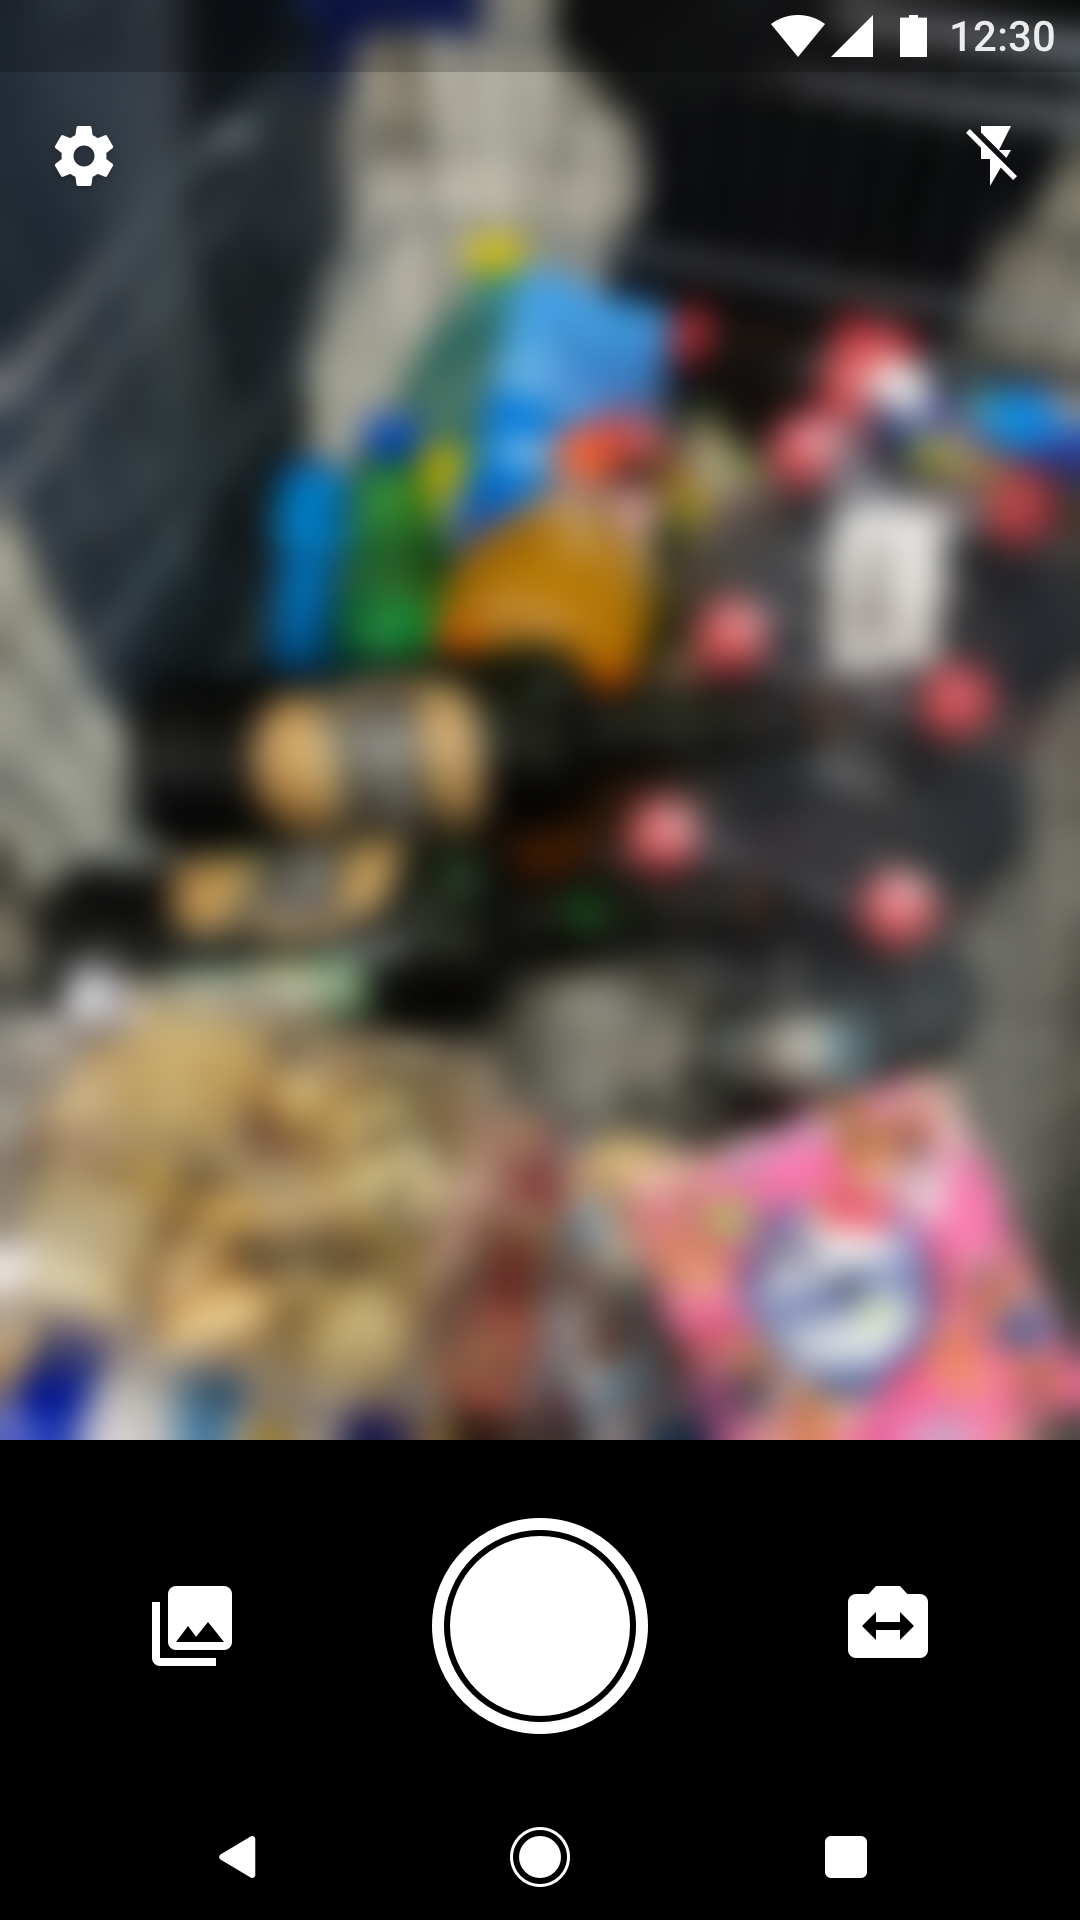
\includegraphics[width=0.4\linewidth]{pics/Artboard}
	\caption{Окно с камерой}
	\label{fig:Artboard}
\end{figure}

На экране с обработанной фотографией по нажатии кнопки «Далее» появляется bottom sheet (рисунок~\ref{fig:Artboard2}), включающий в себя быстрые функции шеринга и сохранения полученного фото в галерею.

\begin{figure}[H]
	\centering
	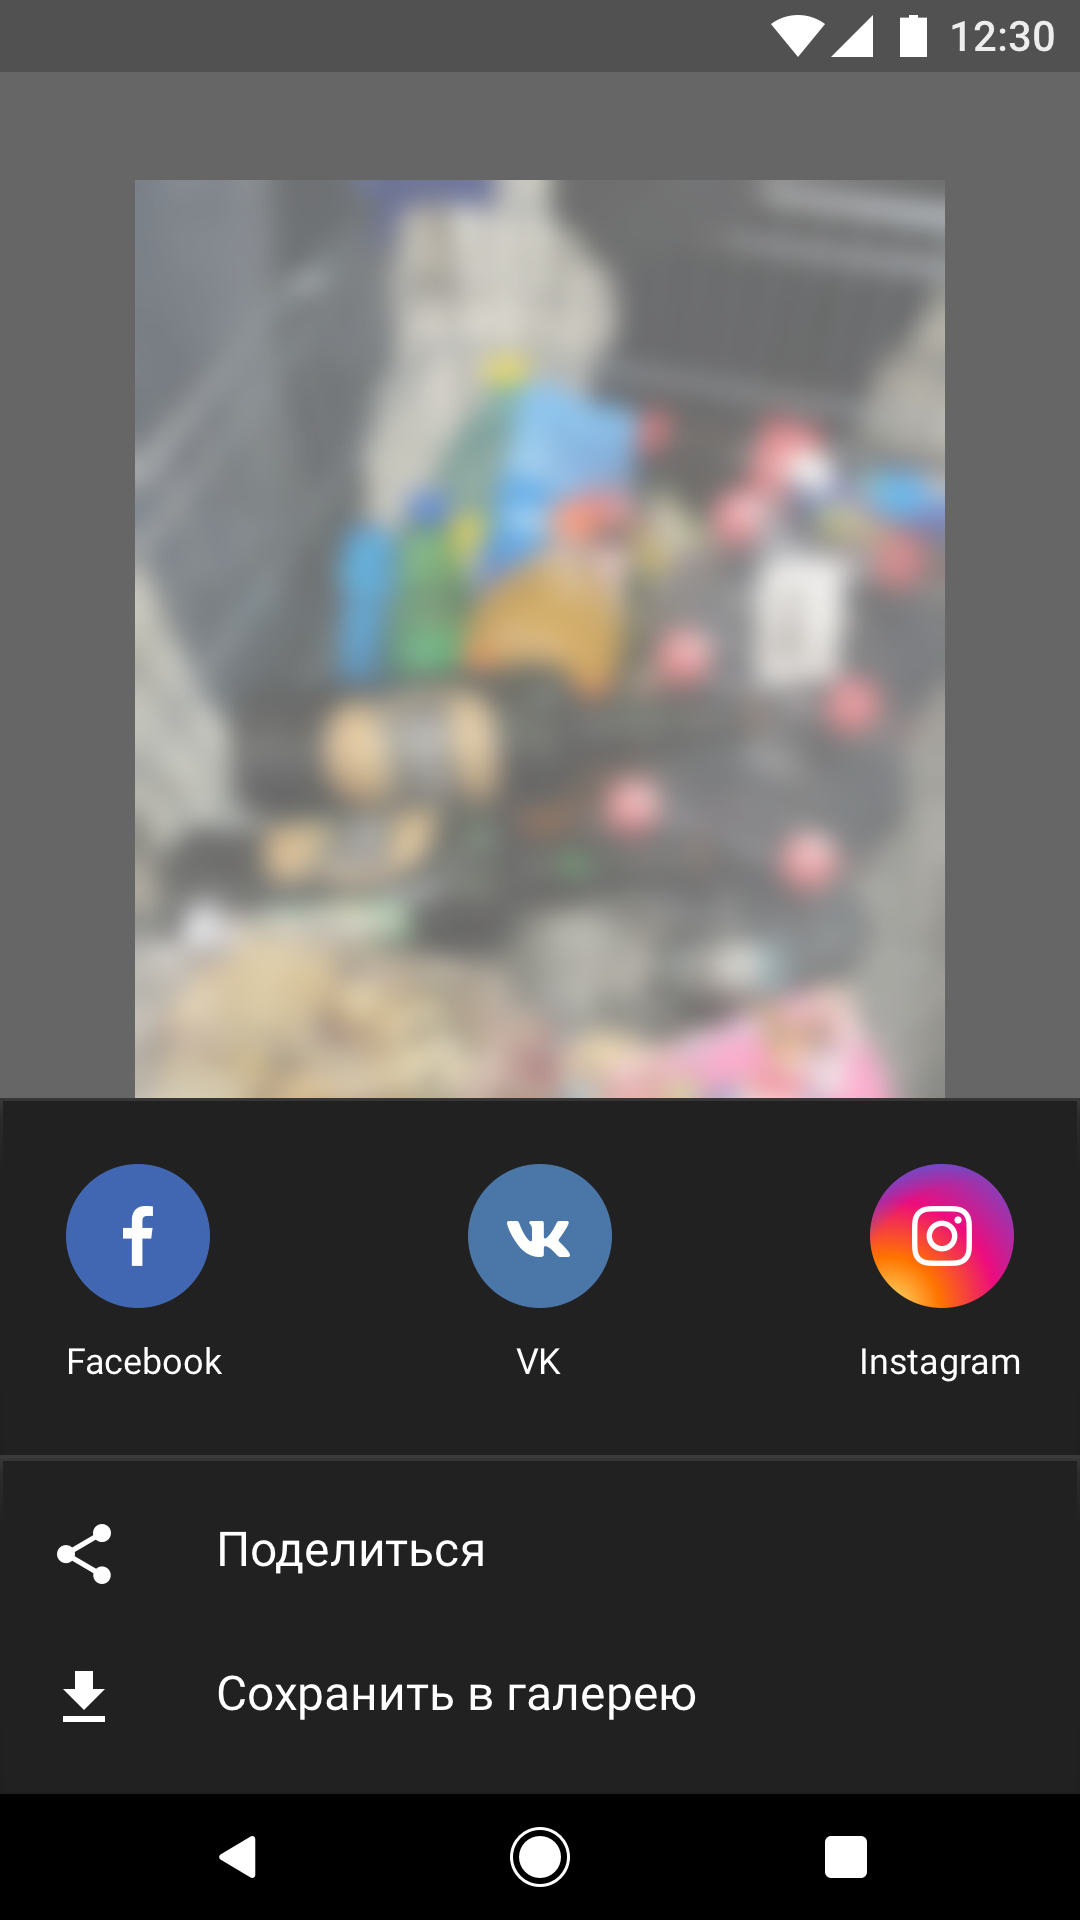
\includegraphics[width=0.4\linewidth]{pics/Artboard2}
	\caption{Окно с просмотром фото}
	\label{fig:Artboard2}
\end{figure}

При создании пользовательского интерфейса приложения были проанализированы современные, с аналогичным функционалом мобильные приложения в целом. Был сделан акцент на необходимости создания современного, функционального и не перегруженного пользовательского интерфейса. В результате проведенного анализа был создан пользовательский интерфейс мобильного приложения для преобразования 2D фотографий в 3D вид.

\subsection{Разработка мобильного приложения}

Рассмотрю практичный пример, когда программно запускаю приложение "Камера", а полученную фотографию сохраняю в папке.~\cite{camera}

В манифесте нужно добавить разрешение на запись файла в хранилище и указать требование наличия камеры.

Используем статическую константу ACTION\_IMAGE\_CAPTURE из объекта MediaStore для создания намерения, которое потом нужно передать методу startActivityForResult(). Разместим на форме кнопку и ImageView, в который будем помещать полученный снимок. Полученное с камеры изображение можно обработать в методе onActivityResult()

При тестировании примера на своём телефоне я обнаружил небольшую проблему - когда снимок передавался обратно на моё приложение, то оно находилось в альбомном режиме, а потом возвращалось в портретный режим. При этом полученный снимок терялся. Поэтому перед нажатием кнопки я поворачивал телефон в альбомный режим, чтобы пример работал корректно. Поэтому надо предусмотреть подобное поведение, например, запретить приложению реагировать на поворот и таким образом избежать перезапуска Activity. 

По умолчанию фотография возвращается в виде объекта Bitmap, содержащего миниатюру. Этот объект находится в параметре data, передаваемом в метод onActivityResult(). Чтобы получить миниатюру в виде объекта Bitmap, нужно вызвать метод getParcelableExtra() из намерения, передав ему строковое значение data.

(рисунок~\ref{fig:my})

\begin{figure}[H]
	\centering
	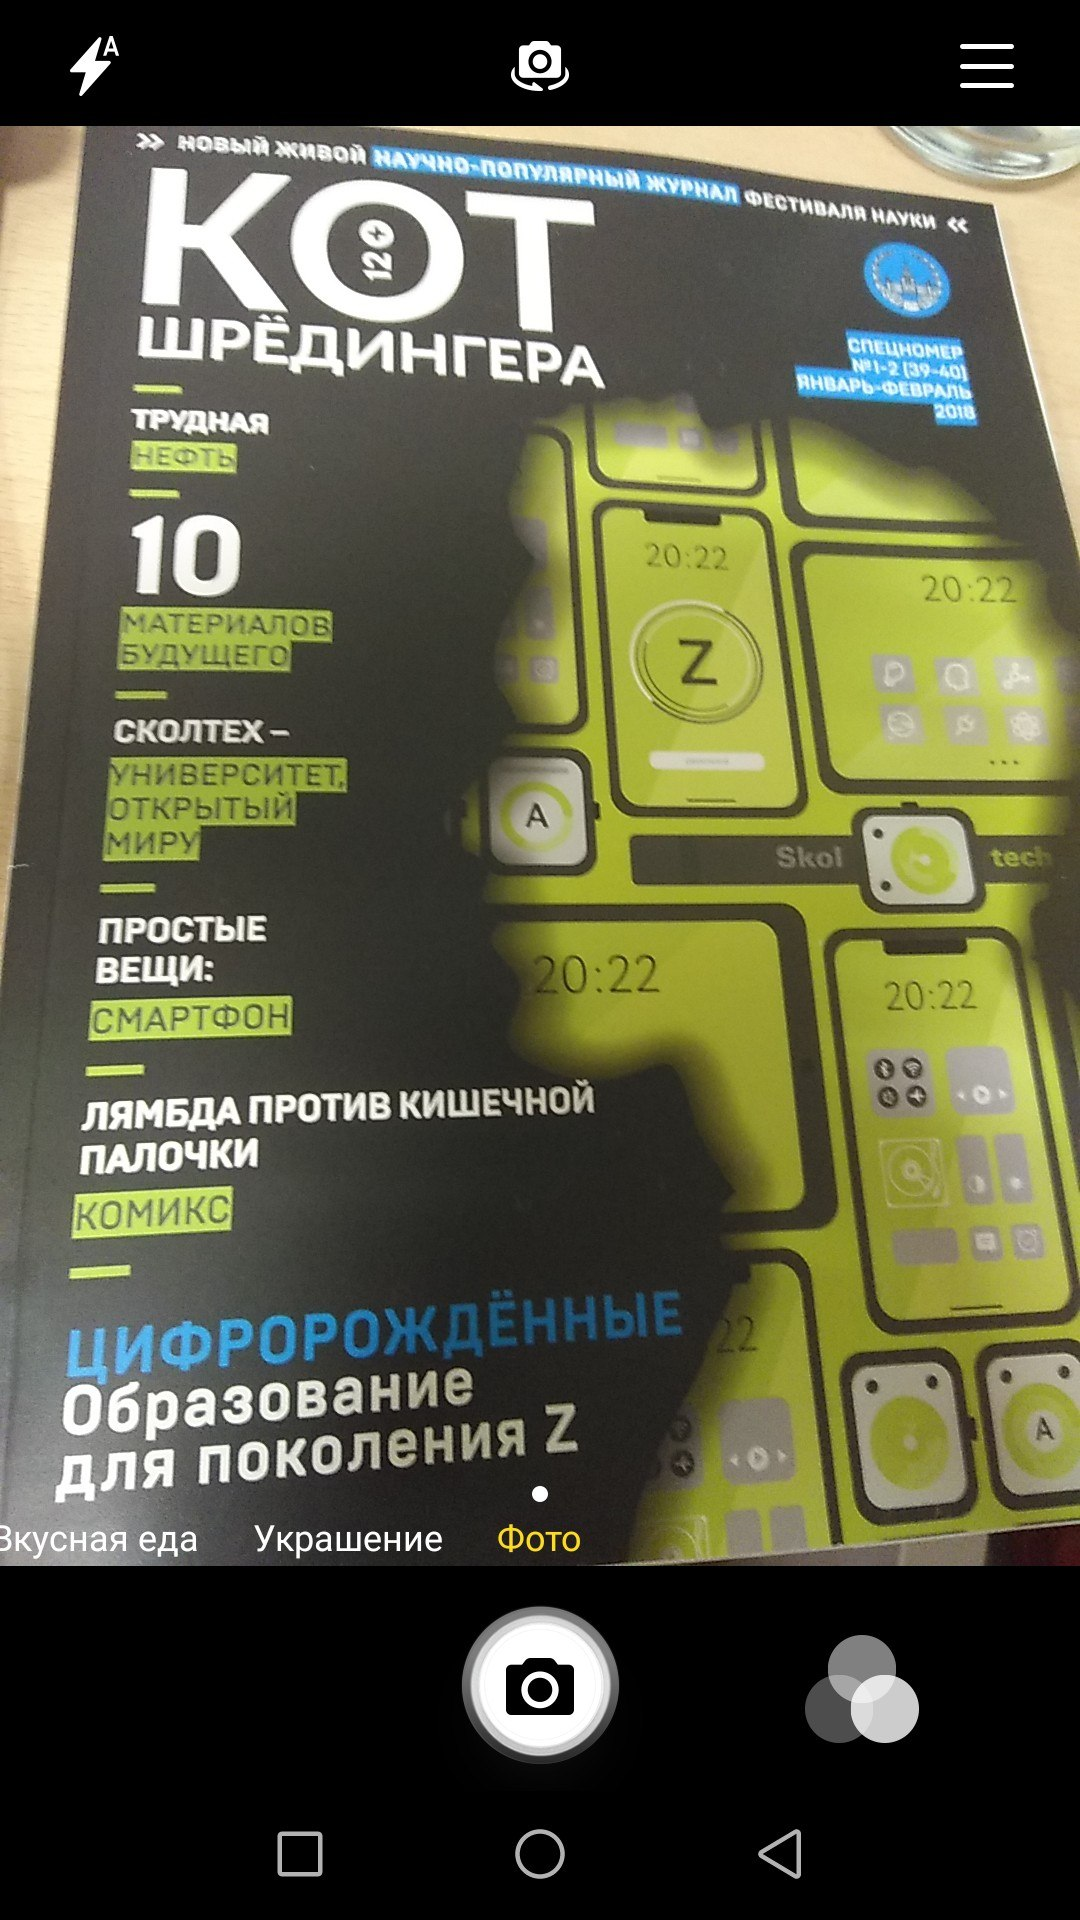
\includegraphics[width=0.4\linewidth]{pics/main}
	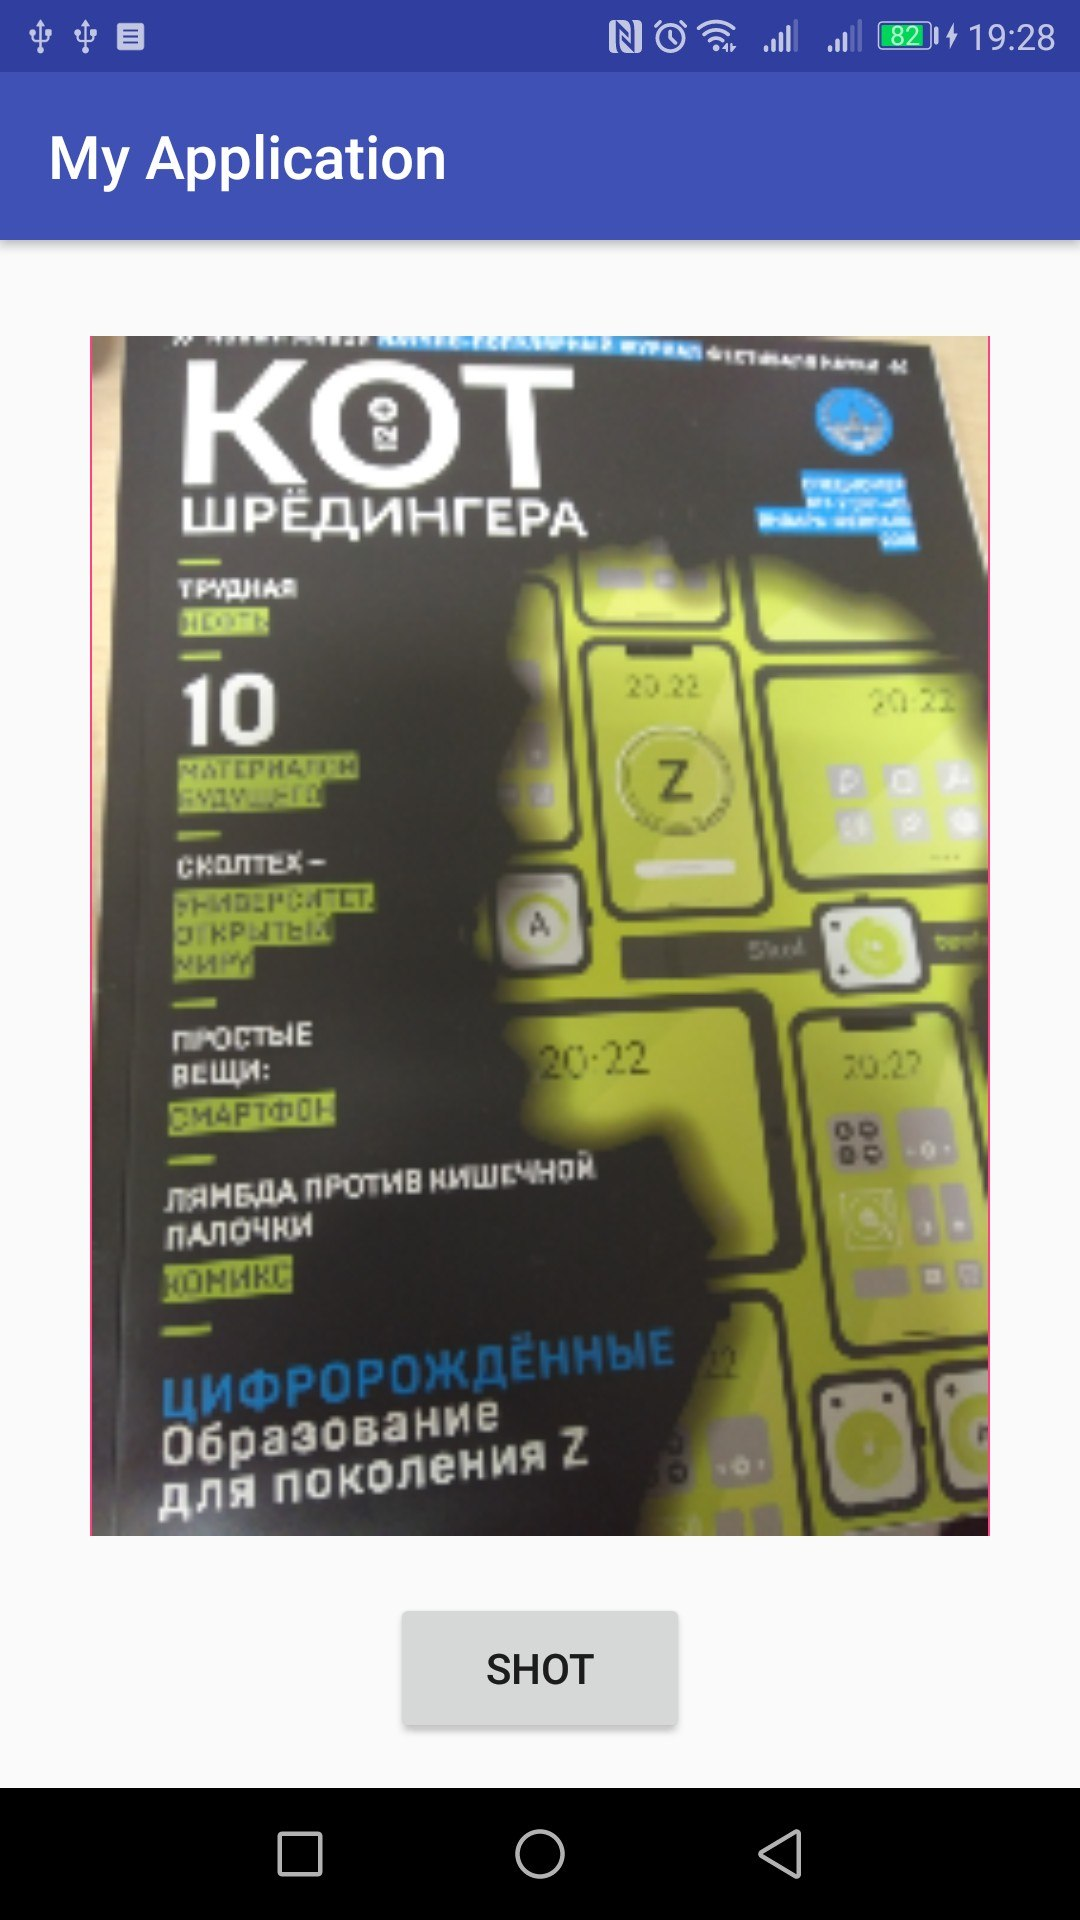
\includegraphics[width=0.4\linewidth]{pics/camera}
	\caption{Результат работы приложения}
	\label{fig:my}
\end{figure}  % первая глава - в файле part1.tex
\pagebreak
% вторая часть

\section{Программная реализация алгоритма преобразования 2D фотографии в 3D}

Рассмотрим сложную задачу восстановления глубины из одного расфокусированного изображения. Входное расфокусированное изображение повторно размыто с использованием гауссова ядра, а значение размытости размытия может быть получено из коэффициента градиента между входными и повторно размытыми изображениями. Распространяя количество размытия в крайних положениях на все изображение, можно восстановить всю карту глубины сцены.

Результат восстановления глубины нашего метода. (рисунок~\ref{fig:input}) Большая интенсивность означает большую глубину на всех картах глубины

\begin{figure}[H]
	\centering
	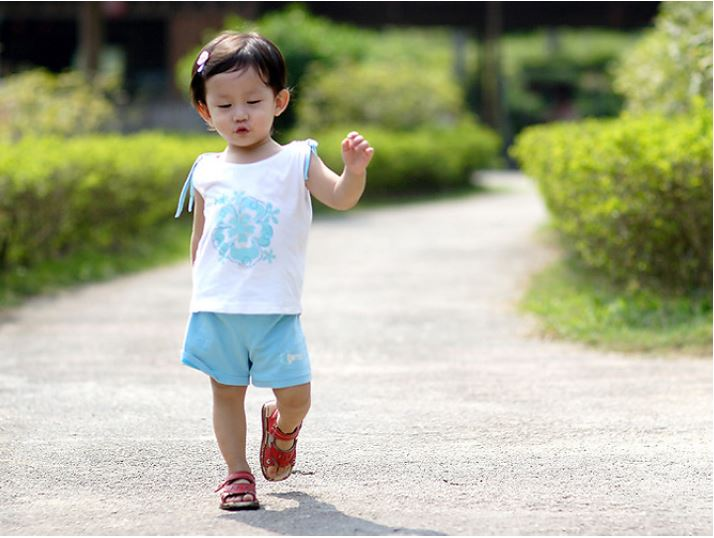
\includegraphics[width=0.4\linewidth]{pics/input}
	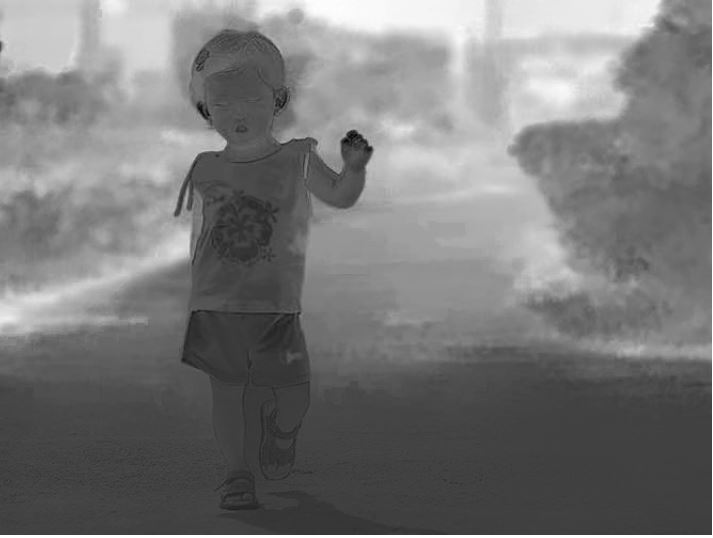
\includegraphics[width=0.4\linewidth]{pics/depth_map}
	\caption{Входное изображение и карта глубины}
	\label{fig:input}
\end{figure}

Сосредоточимся на более сложной проблеме восстановления относительной глубины из одного расфокусированного изображения, захваченного некалиброванной обычной камерой. Метод обратной диффузии~\cite{Proc} моделирует размытие дефокусировки в качестве процесса диффузии тепла и использует неоднородную диффузию тепла для оценки размытости размытия в краевых положениях. В отличие от этого, моделируем размытие дефокусировки как размытие 2D Gaussian. Входное изображение повторно размывается с использованием известного гауссовского размытия, и рассчитывается коэффициент градиента между входными и повторно размытыми изображениями. Величина размытия в краевых местоположениях может быть получена из отношения.

Рассмотрим эффективный метод оценки размытия, основанный на гауссовском градиентном соотношении, и показываем, что он устойчив к шуму, неточному расположению краев и помехам от соседних ребер. Без каких-либо изменений в камерах или при использовании дополнительного освещения наш метод позволяет получить карту глубины сцены, используя только одно расфокусированное изображение, снятое обычной камерой. Как показано (рисунок~\ref{fig:input}), этот метод может извлекать карту глубины сцены с довольно высокой степенью точности.


\subsection{Тестирование стабильности и качества алгоритма}

\begin{figure}[H]
	\centering
	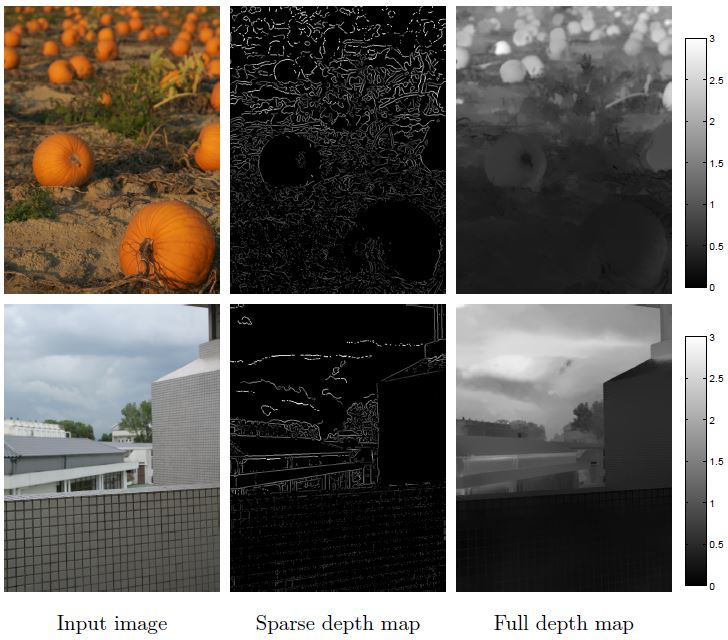
\includegraphics[width=0.7\linewidth]{pics/comparison}
	\caption{Восстановление глубины на реальных изображениях. Наш метод может работать как на сценах с непрерывной глубиной (изображение тыквы), так и на слоистой глубине (изображение здания) для получения карты глубины с довольно хорошей точностью.}
	\label{fig:comparison}
\end{figure}\

Как показано на рисунке~\ref{fig:comparison}, я тестирую наш метод на некоторых реальных изображениях. В изображении тыквы глубина сцены непрерывно изменяется от нижней к верхней части изображения. Оценочная карта глубины фиксирует непрерывное изменение глубины. В изображении здания сцена в основном содержит три слоя: стены, дом и небо. Наш метод позволяет создавать карты глубин, точно представляющие эти слои глубины. Как видно из результатов, наш метод позволяет точно восстановить глубину сцены из одного расфокусированного изображения. На рисунке~\ref{fig:flower} мы сравниваем наш метод с методом обратной диффузии~\cite{Proc}.

\begin{figure}[H]
	\centering
	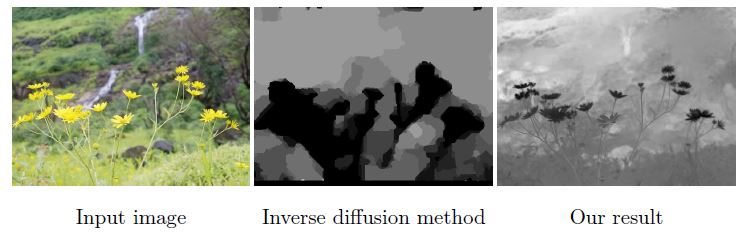
\includegraphics[width=1\linewidth]{pics/flower}
	\caption{Сравнение нашего метода с методом обратной диффузии, на примере цветка}
	\label{fig:flower}
\end{figure}\

Метод обратной диффузии создает грубую слоистую карту глубины. В результате этого цветочный слой плохо отделен фоновыми слоями и содержит некоторые оценки погрешности. Напротив, наш метод способен производить более точную и непрерывную карту глубины, а цветочный слой хорошо отделен фоновой травой и деревьями. % вторая глава - в файле part2.tex
\pagebreak

\section*{\centering ЗАКЛЮЧЕНИЕ}
\addcontentsline{toc}{section}{ЗАКЛЮЧЕНИЕ}

В ходе проделанной работы изучил основы разработки мобильного приложения в среде Android Studio. Также была изучена работа алгоритма определения глубины изображения, протестированы стабильность и качество работы алгоритма преобразования 2D фотографии в 3D.

При создании пользовательского интерфейса приложения был сделан акцент на необходимости создания современного, функционального и не перегруженного пользовательского интерфейса. В результате  было создано мобильное приложение, с помощью которого можно сделать снимок и сохранить его в галерею.

% оформление библиографии - вариант с БД
\pagebreak

\addcontentsline{toc}{section}{СПИСОК ИСПОЛЬЗОВАННОЙ ЛИТЕРАТУРЫ}
% ВАЖНО: для корректного отображения в списке литературы ссылок на англ.языке в bibtex-описание источника следует добавить поле 
% langid = {english}
\printbibliography

\pagebreak



\end{document}          

